%- block legend

\begin{center}
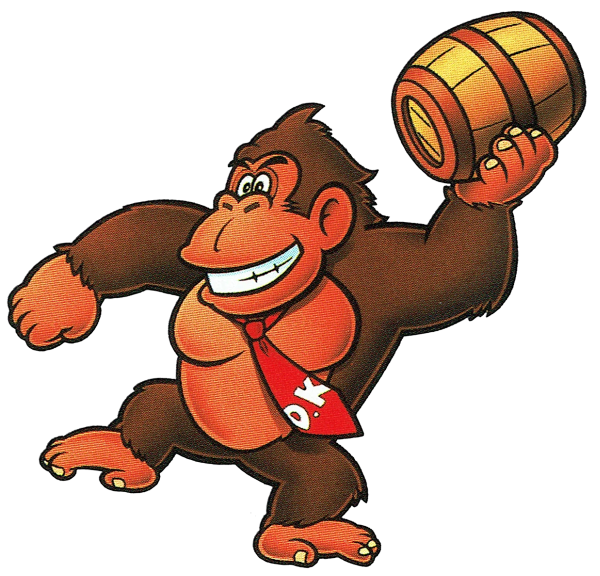
\includegraphics[scale=0.15]{dk.png}
\end{center}

Na Ilha dos Kongs tem $N$ macacos que adoram muito bananas, mas tem o pavio muito curto. Todos na ilha tem um barril com a exata mesma quantidade de bananas que os barris dos outros macacos, pois se um macaco tem mais banana que outro é motivo para confusão!

Uma bela noite enquanto todos os macacos estavam dormindo, o crocodilo \textit{King K. Rool} invadiu a ilha e roubou o barril de alguns macacos. Na manhã seguinte começou o maior alvoroço pois os macacos cujos barris foram roubados agora tinham menos bananas que outros.

Para evitar a briga de se intensificar ainda mais, o ancião da ilha, \textit{Cranky Kong}, propôs a seguinte solução: pegar o total de $B$ bananas que estão distribuidas entre todos os barris que ainda estão na ilha e redistribui-lás igualmente entre todos os macacos. Para isso, \textit{Cranky Kong} precisa de sua ajuda para saber se é possível dividir $B$ bananas entre $N$ macacos de modo que todos tenham a mesma quantidade de bananas.
%- endblock

%- block input
A entrada consiste de dois números inteiros, $N$ e $B$ ($1 \leq N \leq B \leq 10^{5}$), o número de macacos e de bananas respectivamente.
%- endblock

%- block output
A saída deve consistir de apenas um número inteiro, a quantidade de bananas que cada macaco vai ter se elas forem divididas igualmente entre eles, se não for possível esse rearranjo, imprima $-1$.
%- endblock

%- block editorial
Verifique se o número de bananas é divisível pelo número de macacos. Caso seja, imprima $B / N$, caso o contrário, imprima $-1$.

Complexidade: $O(1)$.
%- endblock
